\documentclass{article}

\renewcommand{\thesection}{}
\renewcommand{\thesubsection}{\arabic{section}.\arabic{subsection}}
\makeatletter
\def\@seccntformat#1{\csname #1ignore\expandafter\endcsname\csname the#1\endcsname\quad}
\let\sectionignore\@gobbletwo
\let\latex@numberline\numberline
\def\numberline#1{\if\relax#1\relax\else\latex@numberline{#1}\fi}
\makeatother

\newcommand{\senoide}{\mbox{$y = A\sin{(\omega x + \varphi)}$}}

\usepackage[utf8]{inputenc}

\title{Série de Fourier}
\author{Gustavo Higuchi}
\date{\today}

\usepackage{natbib}
\usepackage{graphicx}
\usepackage{amssymb}
\usepackage{amsthm}
\usepackage{amsmath}
\usepackage{color}   %May be necessary if you want to color links
\usepackage[portuguese, ruled, linesnumbered]{algorithm2e}
\usepackage{pgfplots}
\pgfkeys{/pgfplots/Axis Style/.style={
    width=13.5cm, height=5cm,
    axis x line=center, 
    axis y line=middle, 
    samples=200,
    ymin=-1.5, ymax=1.5,
    xmin=0, xmax=13.0,
    domain=0:4*pi
}}

\usepackage{mathtools}
\DeclarePairedDelimiter\ceil{\lceil}{\rceil}
\DeclarePairedDelimiter\floor{\lfloor}{\rfloor}

% usado para linkar cada section na tabela de conteúdo com a respectiva
% página no documento
\usepackage{hyperref}
\hypersetup{
    colorlinks,
    citecolor=black,
    filecolor=black,
    linkcolor=black,
    urlcolor=black,
    linktoc=all
}

%o começo do documento
\begin{document}

% compila o título
\maketitle

% compila a tabela de conteúdos
\tableofcontents
\newpage


\section{Funções periódicas}
Uma função $f(x)$ é dita periódica se existe uma constante $T > 0$, tal que 
\begin{equation}
\label{prop1}
    f(x + T) = f(x)
\end{equation}
para qualquer $T \in \mathbb{R}$. \\
Essa constante T é chamada de período da função $f(x)$. As funções periódicas 
mais comuns são $\sin{x}$, $\cos{x}$, $\tan{x}$, etc. Funções periódicas surgem
em muitas aplicações matemáticas e em problemas de física e engenharia. Esta 
claro que a soma, a diferença, a multiplicação e a divisão de duas funções 
periódica com período T é também uma função periódica com período T.\\
\\
Se plotarmos o gráfico da função $y=f(x)$ em qualquer intervalo fechado 
\mbox{$a \leq x \leq a + T$}, é possível obter o gráfico de $f(x)$ através da 
repitição periódica da porção do gráfico correspondente a \mbox{$a \leq x \leq a + T$}.\\
\\
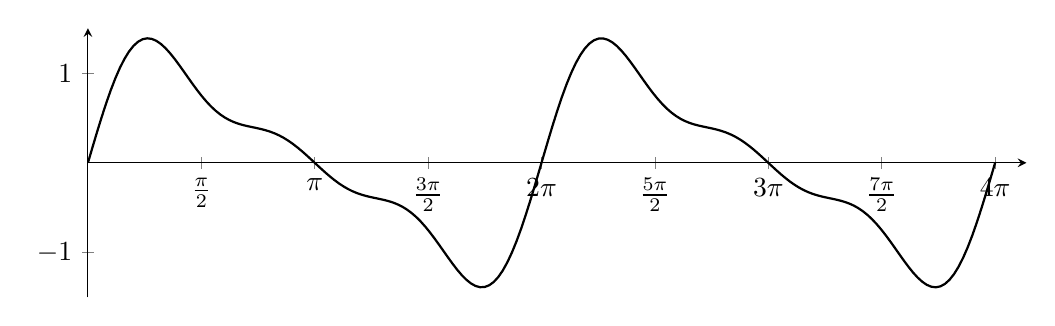
\begin{tikzpicture}
\begin{axis}[
    Axis Style,
    xtick={
        -6.28318, -4.7123889, -3.14159, -1.5708,
        1.5708, 3.14159, 4.7123889, 6.28318, 7.85398,
        9.42478, 10.99558, 12.56638
    },
    xticklabels={
        $-2\pi$, $-\frac{3\pi}{2}$, $-\pi$, $-\frac{\pi}{2}$,
        $\frac{\pi}{2}$, $\pi$, $\frac{3\pi}{2}$, $2\pi$,
        $\frac{5\pi}{2}$, $3\pi$, $\frac{7\pi}{2}$, $4\pi$
    }]
\addplot [mark=none, thick] {sin(deg(x)) + 1/2*sin(deg(2*x)) + 1/4*sin(deg(3*x))};
\label{period_ex}
\end{axis}
\end{tikzpicture} \\
\\
Se $T$ é um período da função periódica $f(x)$, então seus múltiplos $2T$, $3T$, $4T$, etc 
também são períodos da função $f(x)$. Isso é verificado facilmente ao inspecionar 
os gráficos de uma função periódica, ou pela série de igualdades:
\begin{equation}
\label{prop2}
    f(x) = f(x + T) = f(x + 2T) = f(x + 4T) = ...
\end{equation} 
\\
Assim, podemos afirmar que se $T$ é um período, então $kT$ também é, para um 
$k \in \mathbb{N}$, i.e., \textbf{se um período existe, ele não é único}.\\
\\ 
A partir disso, temos a seguinte propriedade de qualquer função periódica $f(x)$
com período $T$:\\
\textit{  Se f(x) é integrável em um intervalo de tamanho T,
então é integrável em qualquer outro intervalo de tamanho T, e o valor da integral
é o mesmo}\\
\begin{equation}
\label{int_prop1}
    \int_a^{a+T} \! f(x) \, \mathrm{d}x = \int_b^{b+T} \! f(x) \, \mathrm{d}x.
\end{equation}
para qualquer a, b. \\
\\
Essa propriedade é uma consequência imediata da interpretação da integral como
área. Cada integral é igual a área incluida entre a curva $y=f(x)$, o eixo x e
as ordenadas desenhadas nos limites do intervalo, onde áreas acima do eixo x
são tidas como positivas, e áreas abaixo são tidas como negativas. No caso,
as áreas representadas pelas duas integrais são a mesma por causa da propriedade 
de $f(x)$.\\
\\
{{gráfico de \ref{int_prop1} }}\\
\\
Daqui em diante, quando uma função $f(x)$ de período $T$ for integrável, então
ela será integrável em qualquer intervalo de tamanho $T$.

\section{Harmonicos}
A função periódica mais simples é $y = \sin{x}$ e pode ser escrito da forma:
\begin{equation}
\label{harm}
    \senoide
\end{equation} 
\\
onde $A$, $\omega$ e $\varphi$ são constantes. Essa função é chamada de função 
de função \textit{harmonica} de amplitude $A$, frequência $\omega$ e fase
inicial $\varphi$. Neste caso, o período dessa harmonica é $T = 2\pi / \omega$
\begin{equation}
\label{harm_ex}
    A\sin{[\omega(x+\dfrac{2\pi}{\omega}) + \varphi]} = A\sin{[(\omega x + \varphi) + 2\pi]} = A\sin{(\omega x + \varphi)}
\end{equation}
\\
{{daí tem uma historinha de onde surgiu esses termos, spoiler: de um problema 
oscilatório.}}\\
\\
Vamos assumir que $\omega > 0$, uma vez que, pela propriedade do seno, $\sin{-a} = - \sin{a}$

Vamos examinar o comportamento da função 
\begin{equation}
\label{harm1}
    \senoide
\end{equation}
\\
Para $A=1$, $\omega = 1$ e $\varphi = 0$, temos a curva senóide comum $y = \sin{x}$\\
\\
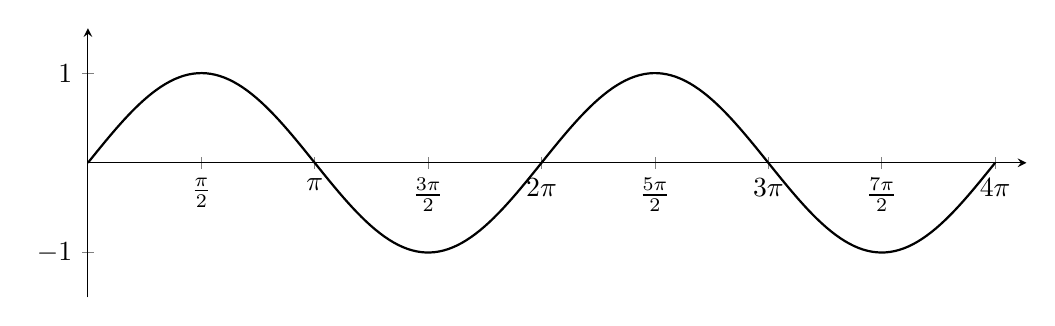
\begin{tikzpicture}
\begin{axis}[
    Axis Style,
    xtick={
        -6.28318, -4.7123889, -3.14159, -1.5708,
        1.5708, 3.14159, 4.7123889, 6.28318, 7.85398,
        9.42478, 10.99558, 12.56638
    },
    xticklabels={
        $-2\pi$, $-\frac{3\pi}{2}$, $-\pi$, $-\frac{\pi}{2}$,
        $\frac{\pi}{2}$, $\pi$, $\frac{3\pi}{2}$, $2\pi$,
        $\frac{5\pi}{2}$, $3\pi$, $\frac{7\pi}{2}$, $4\pi$
    }]
\addplot [mark=none, thick] {sin(deg(x))};
\label{senoide}
\end{axis}
\end{tikzpicture}
\\
Agora considere o seguinte harmonico $y = \sin{wx}$ e definir $\omega x = z$, teremos
$y = \sin{z}$ cujo gráfico é a curva senóide normal. Portanto, o gráfico de 
$y = \sin{\omega x}$ é obtido deformando o gráfico da senóide comum. Por exemplo,
se atribuirmos um $\omega > 1$, teremos uma \textit{compressão} do gráfico da
senóide, então se tivermos $A = 1$, $\omega = 3$ e $\varphi = 0$, o gráfico 
desse harmonico seria como \ref{freq_ex1} abaixo.
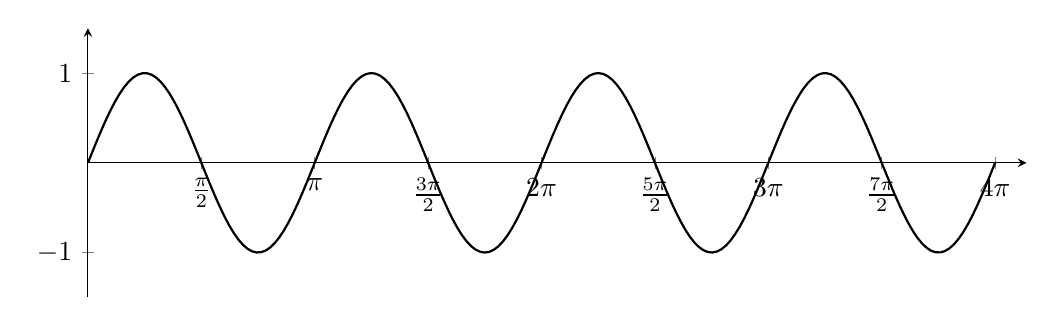
\begin{tikzpicture}
\begin{axis}[
    Axis Style,
    xtick={
        -6.28318, -4.7123889, -3.14159, -1.5708,
        1.5708, 3.14159, 4.7123889, 6.28318, 7.85398,
        9.42478, 10.99558, 12.56638
    },
    xticklabels={
        $-2\pi$, $-\frac{3\pi}{2}$, $-\pi$, $-\frac{\pi}{2}$,
        $\frac{\pi}{2}$, $\pi$, $\frac{3\pi}{2}$, $2\pi$,
        $\frac{5\pi}{2}$, $3\pi$, $\frac{7\pi}{2}$, $4\pi$
    }]
\addplot [mark=none, thick] {sin(deg(2*x))};
\label{freq_ex1}
\end{axis}
\end{tikzpicture}

Ou seja, tivemos uma "compressão" da curva senóide original ao setar $\omega = 2$,
sendo assim sempre que tivermos um $\omega > 1$, teremos uma propocionalmente
\textbf{menor}, neste caso $T = 2\pi / \omega = 2\pi / 3$.

Por outro lado, se atribuirmos um $\omega < 1$, teríamos uma \textit{expansão}
do gráfico da senóide, então se para $A = 1$, $\omega = 1/4$ e $\varphi = 0$,
o gráfico seria:\\
\begin{tikzpicture}
\begin{axis}[
    Axis Style,
    xtick={
        -6.28318, -4.7123889, -3.14159, -1.5708,
        1.5708, 3.14159, 4.7123889, 6.28318, 7.85398,
        9.42478, 10.99558, 12.56638
    },
    xticklabels={
        $-2\pi$, $-\frac{3\pi}{2}$, $-\pi$, $-\frac{\pi}{2}$,
        $\frac{\pi}{2}$, $\pi$, $\frac{3\pi}{2}$, $2\pi$,
        $\frac{5\pi}{2}$, $3\pi$, $\frac{7\pi}{2}$, $4\pi$
    }]
\addplot [mark=none, thick] {sin(deg((x/2))};
\label{freq_ex2}
\end{axis}
\end{tikzpicture}
\\
Assim, teremos uma "expansão" do gráfico da curva senóide original ao setar $\omega < 1$,
e uma função com período \textbf{maior} com $\omega < 1$, neste caso 
\mbox{$T = 2\pi/\omega = \dfrac{2\pi}{1/2} = 4\pi$}.

Agora considere o harmonico $y = \sin{(\omega x + \varphi)}$ e definir $\omega x + \varphi = \omega z$,
para que $x = z - \varphi/\omega$. Como já sabemos o gráfico de $\sin{\omega z}$, o gráfico 
de $y = \sin{(\omega x + \varphi)}$ é obtido deslocando o gráfico de $y = \sin{\omega x}$ ao
longo do eixo x por $-\varphi/\omega$. Então, dado $A = 1$, $\omega = 1$ e $\varphi = 1/2$,
teremos a curva que representa o $\cos{x}$\\
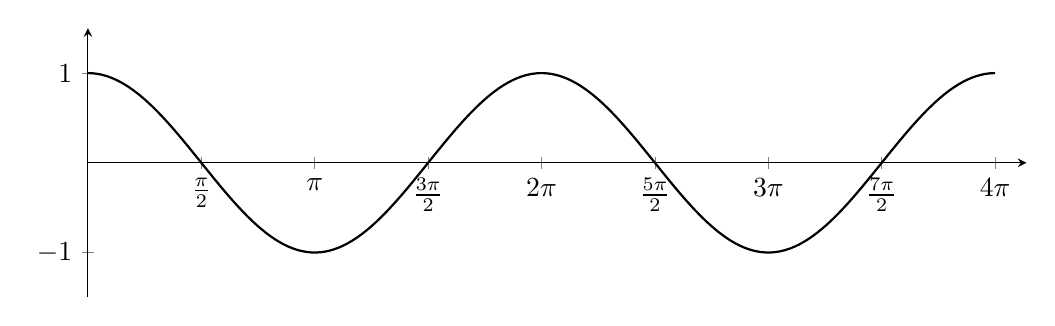
\begin{tikzpicture}
\begin{axis}[
    Axis Style,
    xtick={
        -6.28318, -4.7123889, -3.14159, -1.5708,
        1.5708, 3.14159, 4.7123889, 6.28318, 7.85398,
        9.42478, 10.99558, 12.56638
    },
    xticklabels={
        $-2\pi$, $-\frac{3\pi}{2}$, $-\pi$, $-\frac{\pi}{2}$,
        $\frac{\pi}{2}$, $\pi$, $\frac{3\pi}{2}$, $2\pi$,
        $\frac{5\pi}{2}$, $3\pi$, $\frac{7\pi}{2}$, $4\pi$
    }]
\addplot [mark=none, thick] {sin(deg(x+(pi/2)))};
\label{fase_ex}
\end{axis}
\end{tikzpicture}
\\
que nada mais é que a curva senóide deslocada para esquerda.\\
\\
Finalmente, o harmonico \senoide é obtido do harmonico $y = \sin{(\omega x + \varphi)}$
multiplicando todas as ordenadas por $A$, então dado $A = 2$, $\omega = 1$ e $\varphi = 0$,
temos\\
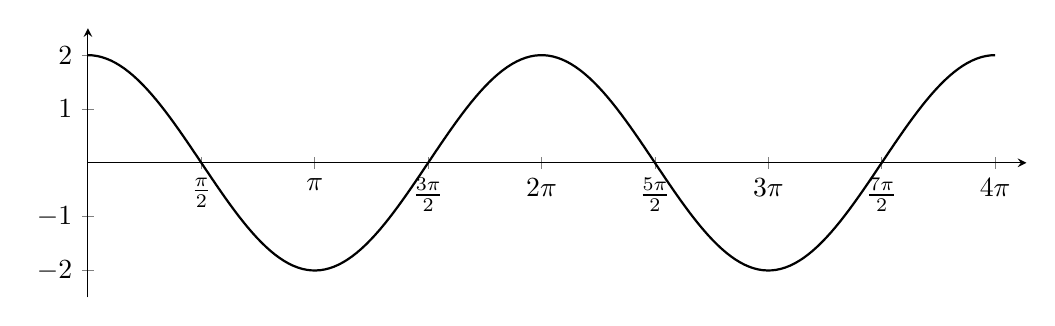
\begin{tikzpicture}
\begin{axis}[
    Axis Style,
    ymin=-2.5,
    ymax=2.5,
    ytick={-2,-1,0,1,2},
    xtick={
        -6.28318, -4.7123889, -3.14159, -1.5708,
        1.5708, 3.14159, 4.7123889, 6.28318, 7.85398,
        9.42478, 10.99558, 12.56638
    },
    xticklabels={
        $-2\pi$, $-\frac{3\pi}{2}$, $-\pi$, $-\frac{\pi}{2}$,
        $\frac{\pi}{2}$, $\pi$, $\frac{3\pi}{2}$, $2\pi$,
        $\frac{5\pi}{2}$, $3\pi$, $\frac{7\pi}{2}$, $4\pi$
    }]
\addplot [mark=none, thick] {2*sin(deg(x+(pi/2)))};
\label{amp_ex}
\end{axis}
\end{tikzpicture}
\\
Portanto, podemos resumir tudo isso no seguinte:\\
\textit{ O gráfico da harmonica \senoide é obtido do gráfico da curva
senóide comum por uma compressão (ou expansão) uniforme ao longo dos eixos,
mais um deslocamento ao longo do eixo x.}\\
\\
Com isso, podemos utilizar uma conhecida fórmula matemática para derivar
o seguinte:\\
\begin{equation}
    A\sin{(\omega x + \varphi)} = A(\cos{\omega x}\sin{\varphi} + \sin{\omega x}\cos{\varphi})
\end{equation}
Então, temos\\
\begin{equation}
\label{ab_harm}
    a = A\sin{\varphi}\text{\hspace{10pt},\hspace{10pt}}b = A\cos{\varphi}
\end{equation}
podemos dizer que todo harmonico pode ser representado na forma
\begin{equation}
\label{eq_harm}
    y = a\cos{\omega x} + b\sin{\omega x}
\end{equation}
\\
Do mesmo jeito que uma função com a forma \ref{eq_harm} é um harmonico também. 
Para provar isso, basta resolver \ref{ab_harm} para $a$ e $b$. O resultado é
\begin{equation}
    \begin{split}
        A = \sqrt{a^2 + b^2}\hspace{5pt},\hspace{10pt} &\sin{\varphi} = \dfrac{a}{A} = \dfrac{a}{\sqrt{a^2 + b^2}}\\
        e\hspace{10pt} & \cos{\varphi} = \dfrac{b}{A} = \dfrac{b}{\sqrt{a^2 + b^2}}
    \end{split}
\end{equation} 
do qual $\varphi$ pode ser facilmente encontrado.\\
\\
Assim, podemos escrever os harmonicos na forma \ref{eq_harm}. No exemplo \ref{amp_ex},
o harmonico pode ser escrito na forma\\
\begin{equation}
    y = \sqrt{2}\cos{3x}+\sin{3x}
\end{equation} 
e essa notação será usada daqui em diante.\\
\\
Também será conviniente explicitar o período $T$ em \ref{eq_harm}. Se definirmos
$T = 2l$, então, como $T = 2\pi/\omega$, temos
\begin{equation}
    \omega = \dfrac{2\pi}{T}=\dfrac{\pi}{l}
\end{equation}

e assim, o harmonico com período $T=2l$ pode ser escrito da seguinte forma\\
\begin{equation}
    a\cos{\dfrac{\pi x}{l}} + b\sin{\dfrac{\pi x}{l}}
\end{equation}

\section{Polinômios trigonométricos e séries}
Dado o período $T=2l$, considere os harmonicos\\
\begin{equation}
    a_k\cos{\dfrac{\pi kx}{l}} + b_k\sin{\dfrac{\pi kx}{l}},\text{\hspace{5pt}para k = 1,2,3,...}
\end{equation}
\\
Com frequencia $\omega_k = k\pi/l$ e períodos $T_k = \dfrac{2\pi}{\omega_k} = \dfrac{2l}{k}$. 
Uma vez que 
\begin{equation}
    T = 2l = kT_k,
\end{equation}  
\\
\textbf{o número $T=2l$ é simultaneamente o período de todos os harmonicos},
pois um múltiplo de um período é também um período (Sec 1). Então, toda soma na 
forma\\
\begin{equation}
    s_n(n) = A + \sum\limits_{k=1}^{n}(a_k\cos{\dfrac{k\pi x}{l} + b_k\sin{\dfrac{k\pi x}{l}}})
\end{equation}
\\
é uma função de período $2l$, uma vez que é uma soma de funções de período 
$2l$. Vale notar que $A$ é uma constante e não afeta a periodicidade da função,
inclusive é possível considerar que uma constante é uma função periódica, onde 
qualquer valor pode ser um período.\\
\\
Essa função $s_n(x)$ é chamada  de \textbf{polinômio trigonométrico de ordem n}(
e período $2l$).\\
\\
Por mais que seja a soma de vários harmonicos, um polinômio trigonométrico pode 
ser usado para representar uma função de natureza muito mais complexa que a 
de um harmonico. E geralmente é o caso. Escolhendo as constantes corretamente,
podemos formar funções com gráficos bem diferentes de um simples harmonico... ?
\textbf{[colocar algumas aplicações mais recentes que "gráficos"]}.
\\
Na primeira figura \ref{period_ex}, o polínomio que representa aquele gráfico é\\
\begin{equation}
    y = \sin{x} + \dfrac{1}{2}\sin{2x} + \dfrac{1}{4}\sin{3x}
\end{equation}
\\
Se colocar em algum software de plot de função, será idêntica à \ref{period_ex}.\\
\\
A \textbf{série trigonométrica infinita}\\ 
\begin{equation}
\label{serie_inf}
    f(x) = A + \sum\limits_{k=1}^{\infty}(a_k\cos{\dfrac{k\pi x}{l}} + b_k\sin{\dfrac{k\pi x}{l}})
\end{equation}
também representa uma função de período $2l$. As funções como \ref{serie_inf} podemos
ser usadas para representar fenômenos de origem muito mais complexa que um polinomio.

Sendo assim, o gráfico de uma função periódica $f(x)$ pode ser obtido através da 
sobreposição de todos os harmonicos que o compõe, i.e., pode ser representado
como uma soma de harmonicos simples.
Então a pergunta que fica é:\\
\textit{Qualquer função que tenha período 2l pode ser representado por uma soma de séries 
trigonométricas?}\\
\\
A resposta é sim, na realidade, é possível ser usado em grande gama classes de problemas!
Diversos outros fenômenos podem ser ser representado por uma série trigonométrica,
tais como......................\\ 
\\
\\  
Se\\
\begin{equation}
\label{serie_longa}
    f(x) = A + \sum\limits_{k=1}^{\infty}(a_k\cos{\dfrac{k\pi x}{l}} + b_k\sin{\dfrac{k\pi x}{l}})
\end{equation}
Então, podemos definir, por comodidade, que $\dfrac{\pi x}{l} = t$ ou que $x = \dfrac{tl}{\pi}$,
assim teremos\\
\begin{equation}
\label{serie_simples}
    g(t) = f(tl/\pi) = A + \sum\limits_{k=1}^{\infty}(a_k\cos{kt} + b_k\sin{kt})
\end{equation}
\\
onde os harmonicos dessa série tenham período $2\pi$. É possível verificar que 
se a função $f(x)$ de período $2l$ possui a expansão \ref{serie_longa}, então
a função $g(x)$ de período $2\pi$ possui a expansão \ref{serie_simples}, e que
o contrário é verdadeiro também. Por ser mais legível, usaremos a expansão 
\ref{serie_simples} e ao final faremos a tradução para o mais genérico 
\ref{serie_longa}.\\

\section{ Uma terminologia mais precisa}
Agora vamos introduzir a uma terminologia mais precisa e relembrar alguns fatos
de cálculo integral e diferencial. Quando dizemos que $f(x)$ é integrável no 
intervalo [a,b], siginifica que a integral\\
\begin{equation}
\label{int}
    \int_{a}^{b}f(x)dx 
\end{equation}
(que pode ser imprópria) existe no sentido elementar. Portanto, nossas funções 
integráveis $f(x)$ sempre serão contínuas ou com finitas descontinuidades no 
intervalo [a,b], no qual a função pode ser limitada ou não.\\
\\
Em cursos de cálculo integral, primeiro se prova que a função possui um número
finito de descontinuidades dentro de um intervalo, então se a integral\\
\\
\begin{equation}
    \int_{a}^{b}|f(x)|dx 
\end{equation} 
\\
existe, então \ref{int} também existe. Neste caso, a função $f(x)$ é tida como
uma função \textbf{absolutamente integrável}. (Vale notar que o inverso pode não
ser verdadeiro).\\
\\
\textbf{Propriedade 1}\\
Se $f(x)$ é uma função absolutamente integrável e $g(x)$ é uma função integrável
limitada, então o produto $f(x)g(x)$ é uma função absolutamente integrável também.
\\
\\
A seguinte regra de integração por partes é válida:\\
\\
\textit{Seja f(x) e g(x) contínuas em [a,b], mas talvez não diferençiavel
em um número finito de pontos. Portanto se f'(x) e g'(x) são absolutamente 
integráveis, então temos:}\\
\begin{equation}
    \int_{a}^{b}f(x)g'(x) dx = [f(x)g(x)]_{a}^{b} - \int_{a}^{b}f'(x)g(x) dx
\end{equation}



\end{document}
